\chapter{Modeling and Model Validation}
\label{modeling}

\begin{figure}[thpb]
      \centering
      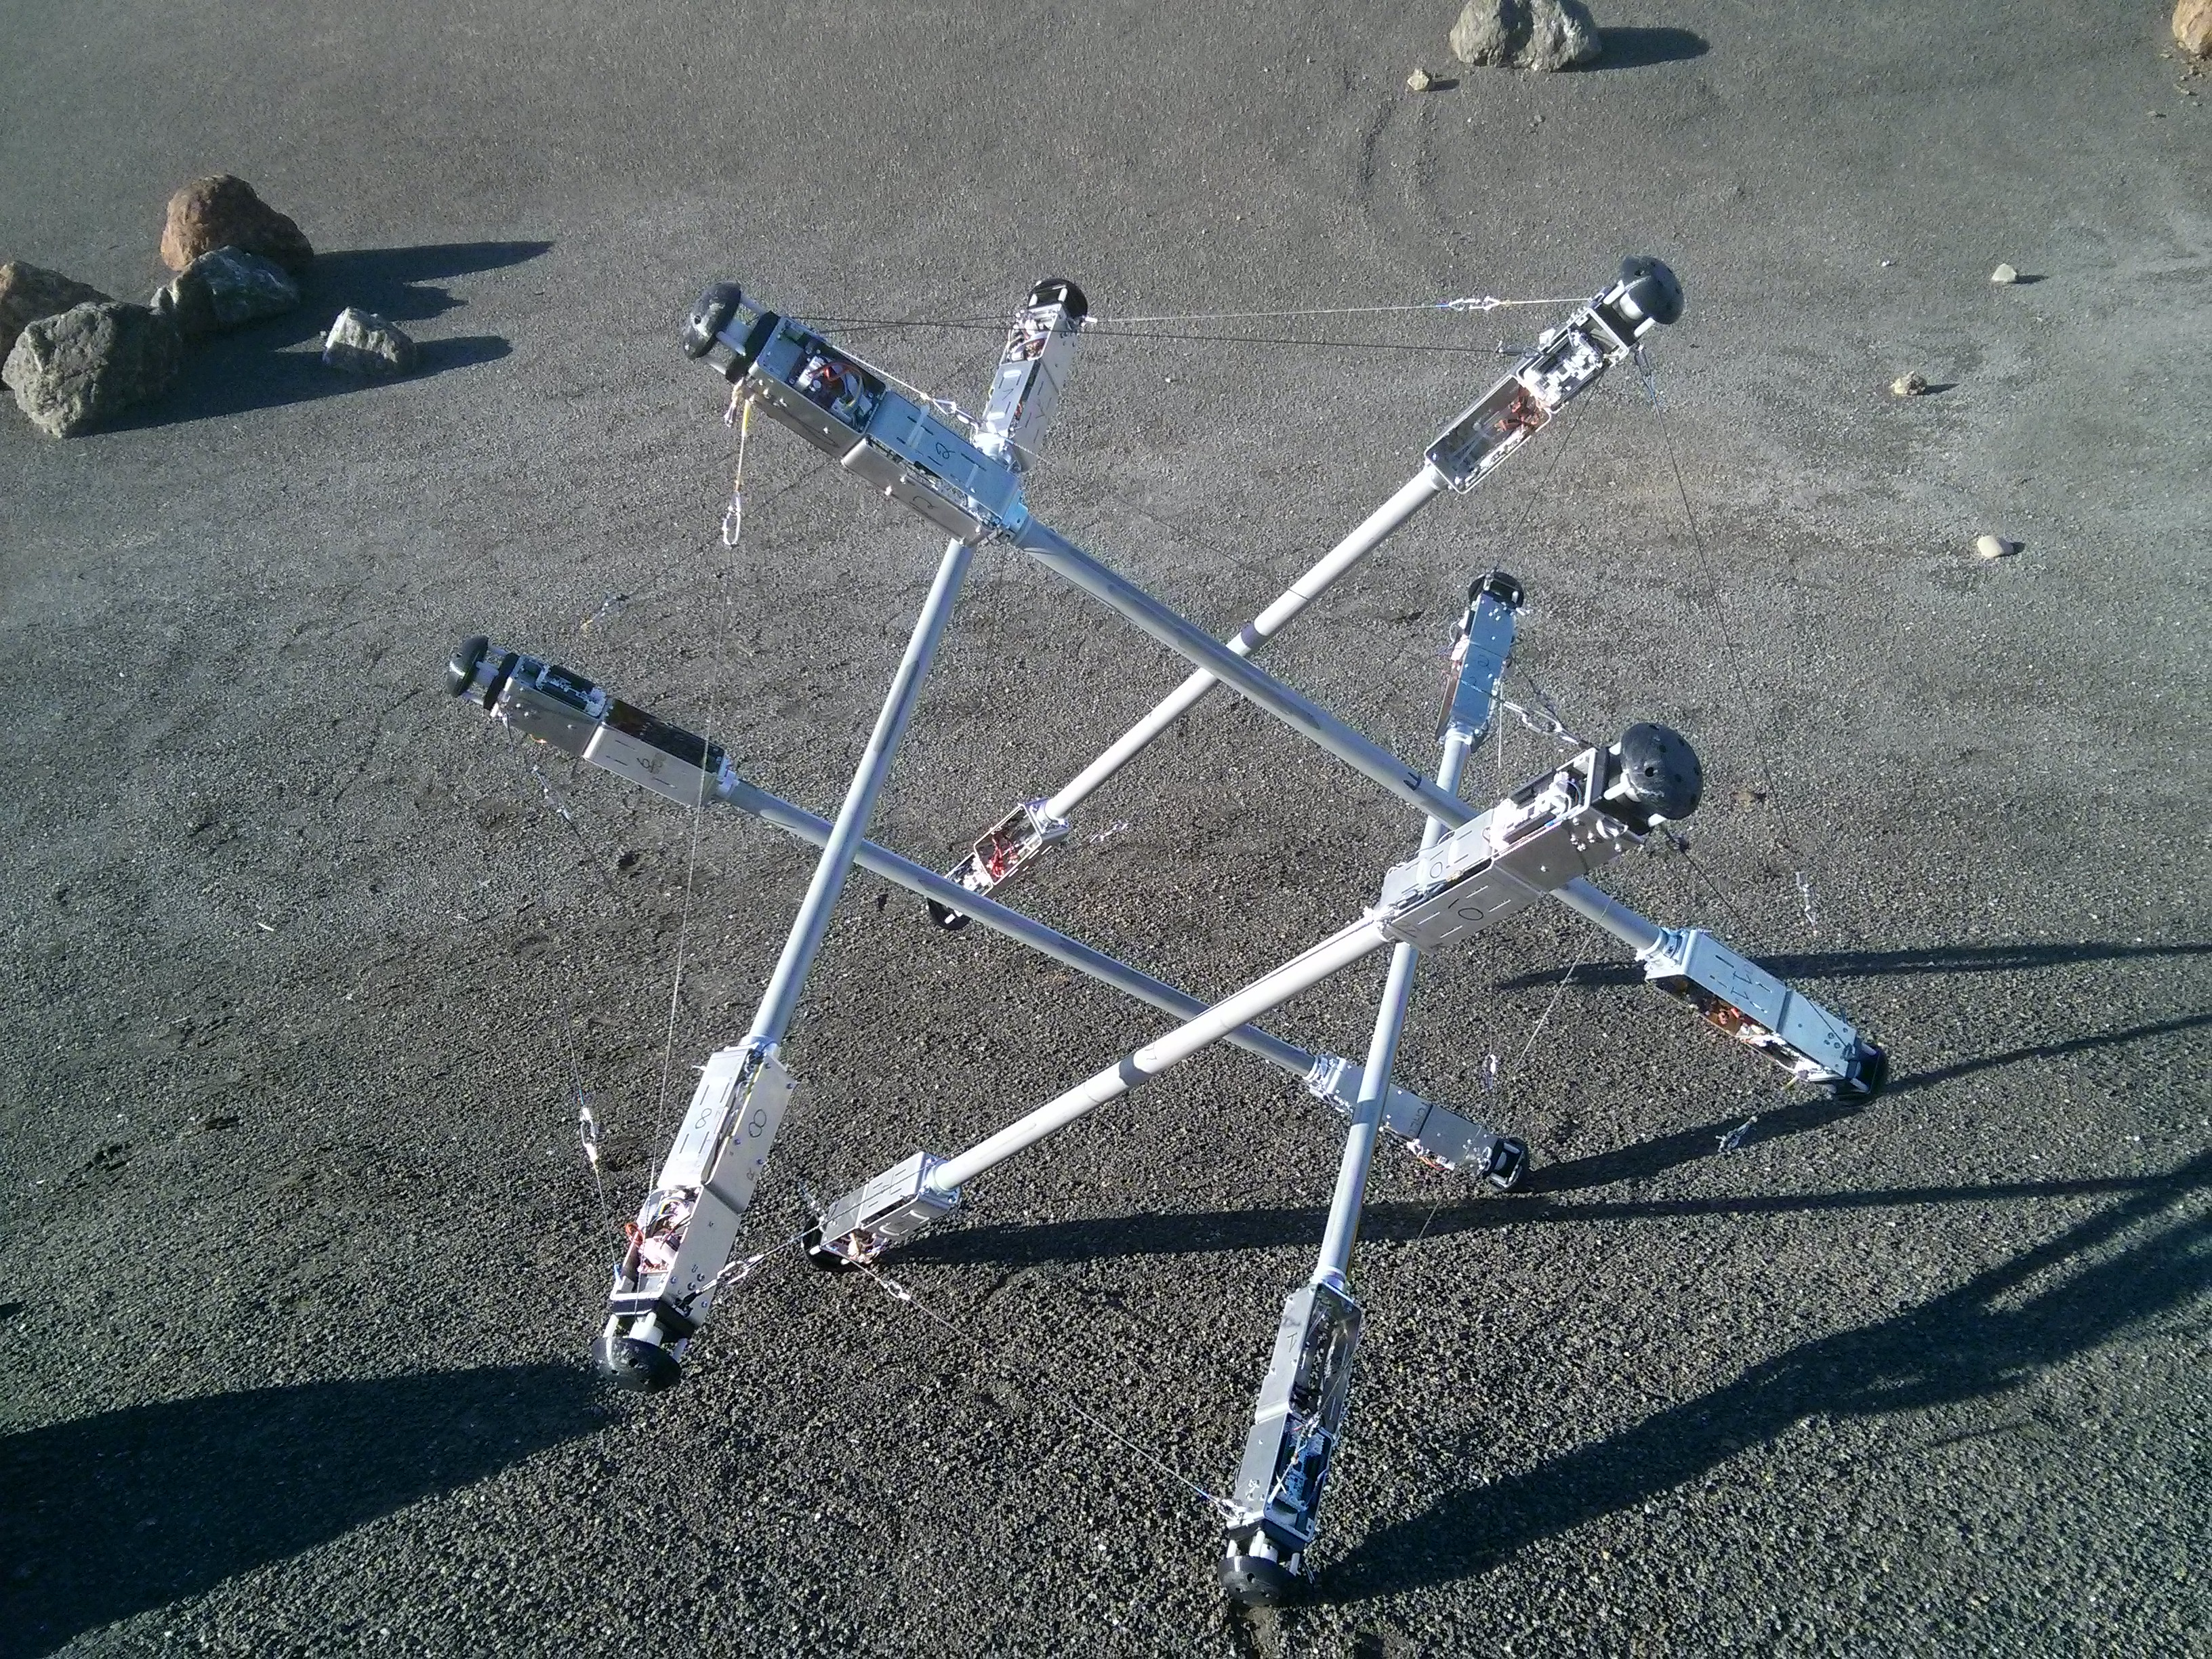
\includegraphics[width=0.8\columnwidth]{tex/img/superball_roverscape2_cropped.jpg}
      \caption{SUPERball, fully assembled, in the NASA Ames Research Center Roverscape.}
      \label{fig:SB}
\end{figure}

As part of our research for the NASA Innovative Advanced
Concepts  (NIAC)  program,  we  are  developing  the \SB{} (Spherical Underactuated Planetary Exploration Robot),
which is a compliant icosahedron tensegrity robot designed
for   planetary   landing   and   exploration, seen in figure \ref{fig:SB}.   Tensegrity   robots
are  soft  machines  which  are  uniquely  able  to  compliantly
absorb  forces  and  interact  with  unstructured  environments.
However, instead of engineering a single new robot, we have
chosen  to  develop  a  fundamentally  reusable  component  for
tensegrity  robots  by  creating  a  modular  robotic  tensegrity
strut which contains an integrated system of power, sensing,
actuation, and communications. The purpose is to enable the
exploration of the wide range of possible tensegrity robotic
morphologies  by  simply  combining  the  robotic  struts  into
new systems.

Though there is much prior work in a variety of theoretical
areas for tensegrities, engineering knowledge of constructing
practical  tensegrity  robots  is  limited.  Since  a  staggering
variety  of  different  tensegrity  structures  can  be  constructed
from  collections  of  simple  sticks  and  strings, we have made it a priority
to develop self-contained robotic tensegrity struts which can
be  used  to  explore  and  build  a  wide  range  of  tensegrity
robots  simply  by  combining  them  into  novel  structures.
Our  designs  are  driven  by  experimental  results  obtained
from  a  previous  prototype,  ReCTeR  (Reservoir  Compliant
Tensegrity Robot) in combination with simulation results of
our validated tensegrity simulator NTRT (NASA Tensegrity
Robotics Toolkit)~\cite{2917079}\cite{Caluwaerts2013rsif}.

In  order  to  develop  SUPERball  from  ReCTeR's  design
limitations as well as our lab’s need for rapid experimentation
of  various  tensegrity  configurations  and  morphologies,  we
came  up  with  a  modular  tensegrity  platform  to  research
large  scale  robotic  tasks;  e.g.  a  tensegrity  planetary  probe
to explore Saturn's moon Titan.
%Our lab obtained design requirements through an iterative
%approach  involving  NTRT  and  ReCTeR.  As  we  validated  our  NTRT  simulator  by  experimental  validation
%with  ReCTeR~\cite{Caluwaerts2013rsif} and can  now  quickly  evaluate  various
Our lab obtained design requirements through an iterative approach with validated our NTRT simulator by experimental comparison with ReCTeR~\cite{Caluwaerts2013rsif}.
We now can quickly  evaluate  various
tensegrity  configurations  in  simulation  to  find  optimal  mechanical  design  goals.  In conjunction with the  NTRT  solver,  we  also
incorporated  results  obtained  with  our  (open  source)  Euler
Lagrange solver based on Skelton's work~\cite{Skelton2009} and measurements on ReCTeR.
The initial design requirements obtained from the NTRT simulations, refined designs after a first prototype build, and how these compare to other tensegrity robotic systems are given in Table \ref{design_req}.


\begin{table*}[ht]
%\begin{minipage}[t][\linewidth]{
\caption{\SB{} and Related Robots Design Overview.} 
\label{design_req}

\begin{center}%
\resizebox{\columnwidth}{!}{%
\begin{tabular}{lrrrcrrrrrrr}
%\hline
&$\bm{l_{strut}}$ & $\bm{\Delta l_{act}}$ & $\bm{k_{passive}}$ & \bf{tethered?} & \bf{control} & $\bm{f_{act}}$ & \bf{\#act.} & \bf{mass} & \bf{sensors} &\bf{actuators} &\bf{ref.} \\ \hline \hline
\bf{Pneumatic}&\SI{.57}{m} & - & - & Y & open loop & \SI{800}{\newton} & \num{24} & \SI{3.3}{\kg}& none & McKibben& \cite{Koizumi2012b} \\
\bf{ReCTeR}&\SI{1}{m} & \SI{0.3}{\metre} & \SI{28.4}{\newton\per\metre} & N & closed loop & \SI{12}{\newton} & \num{6} & \SI{1.1}{\kg} & F, L, IMU & DC & \cite{Caluwaerts2013rsif} \\
\bf{Rapid Proto Kit}&\SI{.69}{m} & \SI{0.005}{\metre} & \SI{1193}{\newton\per\metre} & N & open loop  & $<$\SI{45}{\newton} & \num{24} & \SI{2.7}{\kg}& none & linear DC &\cite{kim2014rapid} \\
\bf{\SB{} 2014}&\SI{1.5}{m} & \SI{0.2}{\metre} & \SI{613}{\newton\per\metre} & N & closed loop & \SI{140}{\newton}  & \num{12} & \SI{12}{\kg}& F, L, $\tau$, IMU & BLDC& \\
\bf{\SB{} 2015}&\SI{1.7}{m} & \SI{0.42}{\metre} & \SI{998}{\newton\per\metre} & N & closed loop & \SI{250}{\newton} & \num{12} & \SI{21}{\kg} & F, L, $\tau$, IMU & BLDC& 
%Tensegrity Kit 
%\SB{} ICRA 2014 &$1.5\mbox{m}$ & $0.26 {\mbox{m}}/{\mbox{s}}$ & $500 \mbox{N}/\mbox{m}$ & $100\mbox{Hz}$ & $3 \mbox{Nm}$ \\
%\SB{} ICRA 2015
%\hline

\end{tabular}
}
\end{center}
\bigskip
\fontsize{10pt}{12pt}\selectfont
The variable $l_{strut}$ indicates the length of a strut, $\Delta l_{act}$ is the nominal spring-cable retraction length in tension, $k_{passive}$ is the linear stiffness coefficient of a passive spring-cable (or active spring-cable if fully actuated), tethered indicates if the robot is powered externally or by internal systems, control indicates whether sensor feedback is used, $f_{act}$ is the nominal actuated spring-cable tension and \#act. is the number of actuators. In the sensors column, F represents a linear force sensor (for cables), L is cable length sensor (in the form of motor encoders), $\tau$ represents a torque sensor for motors, and IMU represents an accelerometer/gyroscope inertial motion sensing unit. Actuators are specified as DC motors or brushless DC (BLDC) motors. The SUPERball 2014 values are revised original design requirements based on NTRT simulations, and changed to the 2015 values after additional detail design. %

\vspace{-0.2cm}

%\end{minipage}
\end{table*}

The work presented here is work verifying our in house tensegrity simulators.
In order to achieve this, the group decided to use a \SB{} like structure with a center payload.
This is believed to be closer to the proposed build profile of a real tensegrity probe, where the main science modules will be contained within the payload.
Protecting this science payload is the main goal for and EDL scenario.
Figure \ref{fig:NTRT_SB} shows a 3-D representation of \SB{} with a payload generated within NTRT.

\begin{figure}[thpb]
      \centering
      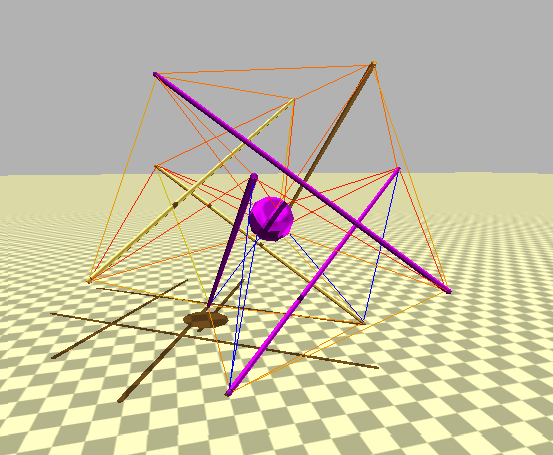
\includegraphics[width=0.8\columnwidth]{tex/img/1.png}
      \caption{SUPERball with a payload modeled within NTRT.}
      \label{fig:NTRT_SB}
\end{figure}

\section{Euler-Lagrange Model}
In order to verify the simulation results produced by our NTRT simulator, we decided to compare the behavior of the NTRT to a published analytic model for tensegrity systems.
We choose to use Skelton's dynamic equations because it is a well accepted and used model.
It may be found in his \emph{Tensegrity Systems} book \cite{skelton_tensegrity_2009} which is based on his work in \cite{skelton2005dynamics}.
In order to solve the dynamic equations with interactions with the environment, an Euler-Lagrange approach is used as well as Skelton's constrained class one structure.
The lagrange equation for a constrained rod is given by
\begin{equation}
\label{eq:lagrange}
L = T - V - c
\end{equation}
where
\begin{align}
\mathbf{b} &= l^{-1}(\mathbf{n}_{j}-\mathbf{n}_{i})\label{eq:normalizedVector}\\
c &= \frac{\mathbf{J}\xi}{2}(\mathbf{b}^{T}\mathbf{b}-1)\label{eq:constraint}
\end{align} 
Equation \eqref{eq:normalizedVector} is the normalized vector of a rod with \(\mathbf{n}_{i,j}\) the nodal positions in \(R^3\), and equation \eqref{eq:constraint} contains the lagrange multiplier \(\xi\) to keep \eqref{eq:normalizedVector} constrained.
\(\mathbf{J}\) is also defined as the inertia matrix for a one dimensional rod in three dimensional space.
In order to define the system of \(k\) rods we need to define a combined Lagrangian as
\begin{equation}
\mathbf{L} = \sum_{i=1}^{k} L_{i}\label{eq:combinedLagrangian}
\end{equation}
where \(L_{i}\) is the Lagrange function for each rod.
Using the approach outlined in Skelton's book for deriving the equations of motion, we can then derive the configuration matrix
\begin{equation}
\mathbf{Q} = \begin{bmatrix}
	\mathbf{R} & \mathbf{B}
	\end{bmatrix}\label{eq:configMatrix}
\end{equation}
where \(\mathbf{R}\) and \(\mathbf{B}\) are matrices containing the translational and rotational vectors, respectively. They have the form
\begin{align}
\mathbf{R} &= \begin{bmatrix}
	\mathbf{r}_{1} & \cdots & \mathbf{r}_{k}
	\end{bmatrix}\label{eq:transR}\\
\mathbf{B} &= \begin{bmatrix}
	\mathbf{b}_{1} & \cdots & \mathbf{b}_{k}
	\end{bmatrix}\label{eq:rotB}
\end{align}
Also using the procedure to derive generalized forces within Skelton's book, the systems's generalized force equations are computed as
\begin{equation}
\mathbf{F}_{\mathbf{Q}} = \begin{bmatrix}
	\mathbf{F}_{\mathbf{R}} & \mathbf{F}_{\mathbf{B}}
	\end{bmatrix}\label{eq:generalizedForce}
\end{equation}
with
\begin{align}
\mathbf{F}_{\mathbf{R}} &= \begin{bmatrix}
	\mathbf{f}_{\mathbf{r}_{1}} & \cdots & \mathbf{f}_{\mathbf{r}_{k}}
	\end{bmatrix}\label{eq:gForceR}\\
\mathbf{F}_{\mathbf{B}} &= \begin{bmatrix}
	\mathbf{f}_{\mathbf{b}_{1}} & \cdots & \mathbf{f}_{\mathbf{b}_{k}}
	\end{bmatrix}\label{eq:gForceB}
\end{align}
Finally, we can define the resulting equations of motion in a compact form as
\begin{equation}
(\ddot{\mathbf{Q}} + \mathbf{Q}\mathbf{\Xi})\mathbf{M} = \mathbf{F}_{\mathbf{Q}}\label{eq:compactForm}
\end{equation}
where
\begin{align}
\mathbf{\Xi} &= diag\begin{bmatrix}
	0,\cdots,0,\xi_{1},\cdots,\xi_{k}
	\end{bmatrix}\label{eq:lagrangeMatrix}\\
\mathbf{M} &= diag\begin{bmatrix}
	m_{1},\cdots,m_{k},J_{1},\cdots,J_{k}
	\end{bmatrix}\label{massMatrix}
\end{align}
This approach was then implemented in Python utilizing a 4th order Runge-Kutta formula for solving the system of ordinary differential equations.  
In order to implement a gravitational field, a force distribution function is applied along the length of each rod and calculated as a nodal force depending on the given density of the rod.
This external force is then applied to the nodes during each time step, simulating a gravitational field.

\section{Detailed Impact Simulations and Cross-Validation Using Two Simulators}
The NTRT simulator is the most general purpose, allowing us to explore control algorithms and complex environmental interactions, but it is an iterative discrete solver that we were concerned might not be providing accurate answers.  The E-L solver, on the other hand, has a much stronger analytical basis and should provide very accurate answers, but is limited because some of the nodes (rod ends) must be constrained and locked into place.  This is unrealistic for the deformation caused during landing, and makes it an inappropriate choice for mobility and controls research.
If ground contact forces are incorporated into the E-L solver and code optimization implemented, it could be used in conjunction with a unscented kalman filter for state estimation propogation.
This tool could then be used to develop online learning algorithms for mobility research.

In this section, we compare the NTRT simulator and E-L solver at the moment of impact with the ground. 
The simulations are compared at the moment of impact with the ground because our implementation of the analytic E-L solver requires select nodes to be constrained.
We setup the structure so that it is barely in contact with the ground and is in balance at time equal to 0. 
In both simulations, we add an initial velocity equal to the terminal velocity of Titan, and compared each vertical trajectory, vertical velocity, and vertical acceleration of the payload. 
Since the structure's horizontal speed is zero at the beginning and the structure is symmetrical, the payload's horizontal components of position, velocity and acceleration are zero. 
As it can be seen in the Figures \ref{fig:vsPosition} and \ref{fig:vsVelocity}, both simulators closely match and generate the same results for position and velocity with the error margin close to zero. 
Comparing the accelerations generated by two simulators (Figure \ref{fig:vsAccelerations}), it can be seen that there is a bigger difference. 
The reason behind this difference is the fact that NTRT uses Bullet, which is a discrete time simulator and accelerations are calculated using two point estimations from velocities at the timestep before.  Yet, even with these differences in accelerations, our conclusion at the end of the comparison is that both simulators showed the same basic dynamics and their results were close enough that we could move forward using the more general purpose NTRT Simulator for our controls, mobility, and landing experiments.


\begin{figure}[htb]
   \centering
   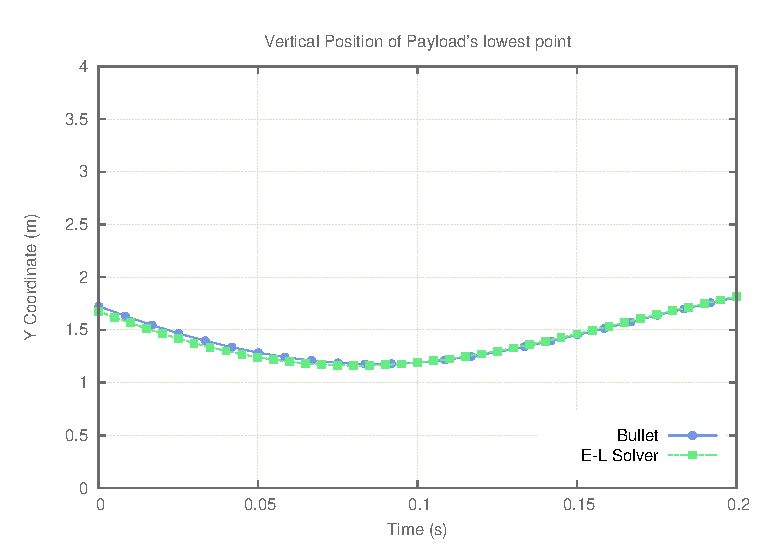
\includegraphics[width=0.8\columnwidth]{tex/images/landing/bulletVsEL/SimVsEL}
   \caption{NTRT vs EL: Vertical Position}
   \label{fig:vsPosition}
\end{figure}

\begin{figure}[htb]
   \centering
   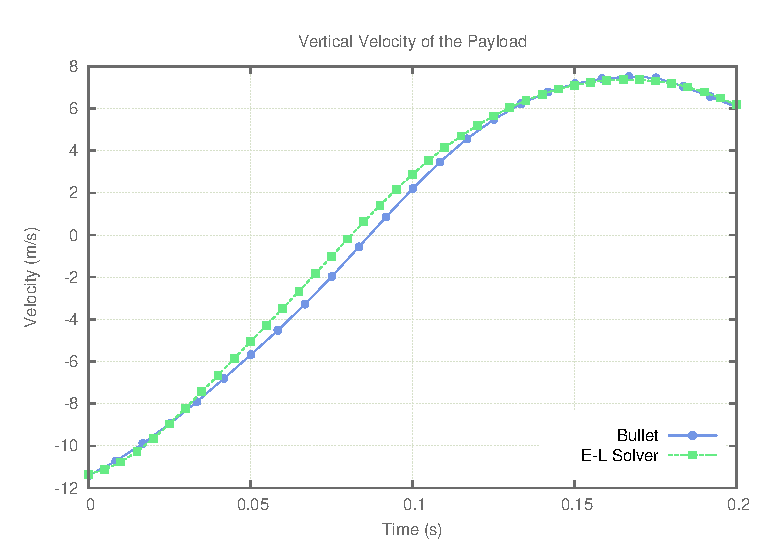
\includegraphics[width=0.8\columnwidth]{tex/images/landing/bulletVsEL/Velocities}
   \caption{NTRT vs EL Vertical Velocity}
   \label{fig:vsVelocity}
\end{figure}
\begin{figure}[htb]
   \centering
   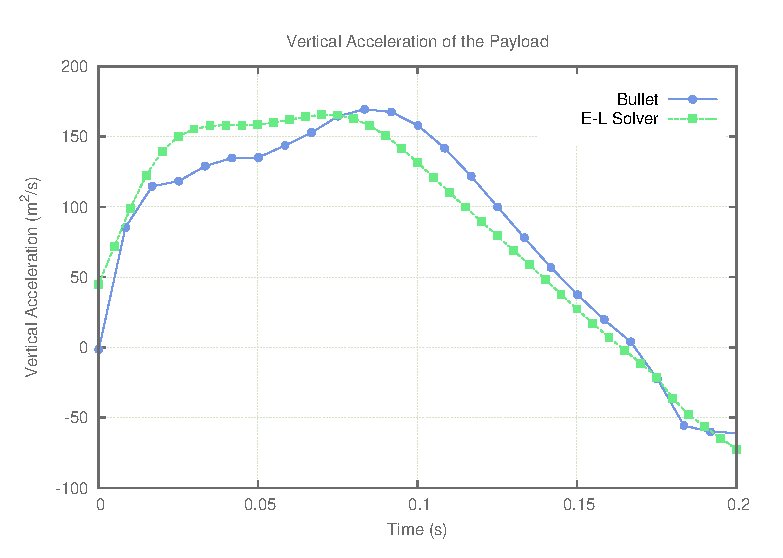
\includegraphics[width=0.8\columnwidth]{tex/images/landing/bulletVsEL/VelocityDerivatives_SimVsEL}
   \caption{NTRT vs EL Vertical Acceleration}
   \label{fig:vsAccelerations}
\end{figure}


\section{Simulated Drop Tests and Payload Protection}

Finally, we performed extensive analysis on drop tests and the protection provided to a payload.   As expected, we found that by varying the rod lengths, which impacts the stroke distance for the payload to decelerate, we could control the maximum deceleration experienced by the payload while ensuring that it did not collide with the ground or structure.  For example, with rods of 1.5 meters in length, our payload experienced a max deceleration of 21.4G when landing at 15 m/s. In figure \ref{fig:rodvsG} we show the results of a series of drop tests with different rod lengths and show the resulting maximum deceleration and forces experienced in the tension members.   As can be seen from these graphs, even for reasonable rod lengths, the maximum G's are acceptable for most instruments, and the maximum forces experienced by the cables are easily within ranges that can be engineered for.  In all tests we kept the total system mass constant, at 100kg (which is 70kg for the payload and 5kg per rod) in order to highlight the impact of structural geometry and rod length.  For the tension members we used spring constants of 44 kN/m for the cables around the perimeter and 10 kN/m for the cables attached to the payload.  Also, the results in Figure \ref{fig:rodvsG} were found using the landing orientation of 35 degrees around X axis and 45 degrees around Z axis, which we selected from our orientation studies discussed below. 

\begin{figure}[htbp]
\centering
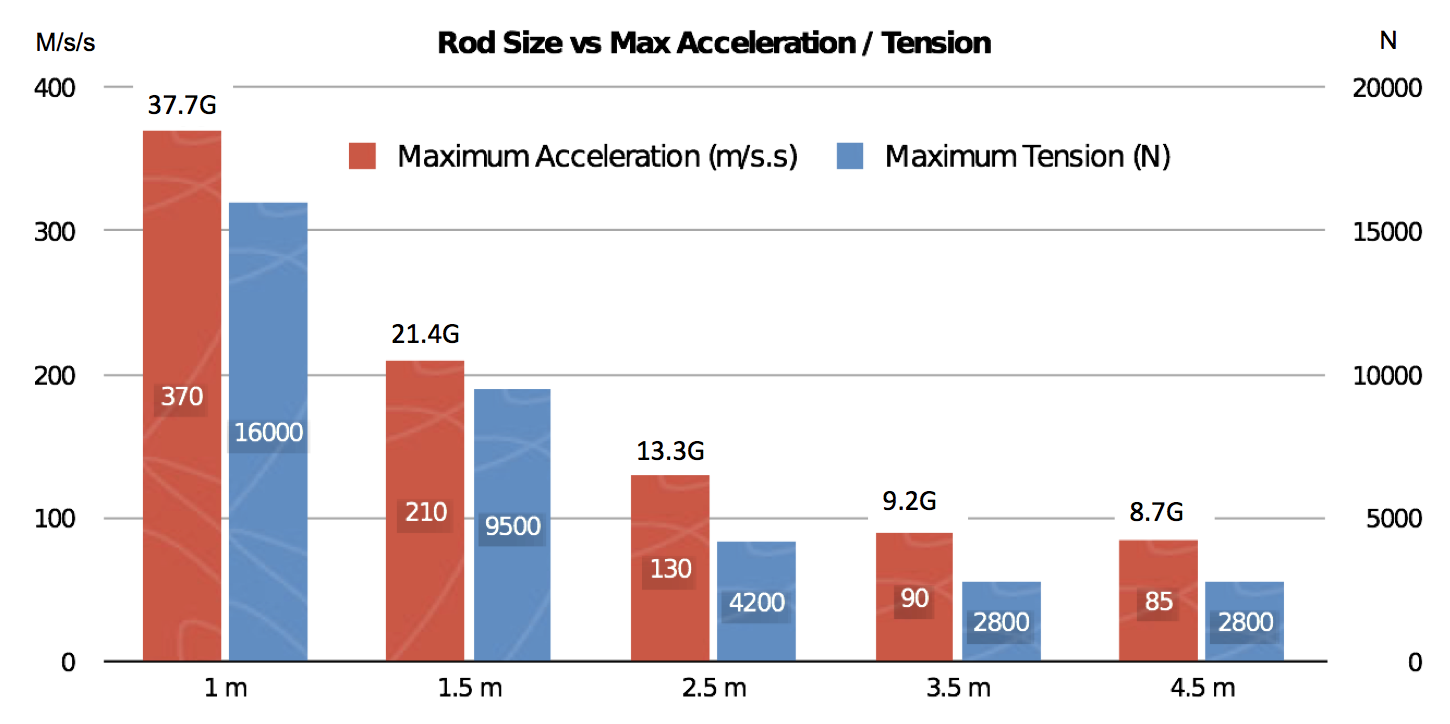
\includegraphics[width=0.8\columnwidth]{tex/images/rodvsG_fixed2}
\caption{{\em {\bf Landing Forces Study}. This shows how rod length impacts maximum deceleration of the payload and  the maximum forces experienced by the tension cables.  All tests were conducted with a landing velocity of 15 m/s onto a hard surface.}}
\label{fig:rodvsG}
\end{figure}

A very interesting point to consider is that the mass of our system will grow in a linear fashion with the length in the rods, while providing increasing payload protection.  On the other hand, the mass of airbags increases with the square of the radius, which is one of the reasons that the MSL rover, with its increased size and mass, had to switch from the airbag approach to the more complex Sky Crane approach.  While this study has focused on small light-weight mission concepts, we expect that there are compelling advantages to scaling up to handle larger payloads and we look forward to studying this further in the future.

\section{Landing Orientation Studies}
In order to study how landing orientation affects payload decelerations and impact events, we conducted a systematic study of landing orientations.  Since we wanted to get meaningful data, even for bad orientations, we used a larger tensegrity with 4 meter rods so the data wouldn't saturate.  Our success criteria for this study was that the decelerations had to stay under an upper limit of 25G deceleration of the payload, and the payload had to avoid collision with the ground or parts of the tensegrity structure.  Figure \ref{fig:landingHeatMapRot} shows the orientations that were safely within these criteria (black) or failed one or both of the criteria (colored).  By using a simple trailing streamer during descent it would be possible to control landing at an optimal orientation and enable the use of smaller structures with shorter rods because the orientation control would maximize the available stroke for the payload to decelerate within the structure.  Conversely, we can use these studies to know what the worst possible landing scenario will be and choose a structure size which will allow safe landing at any orientation.

\begin{figure}[htbp]
   \centering
   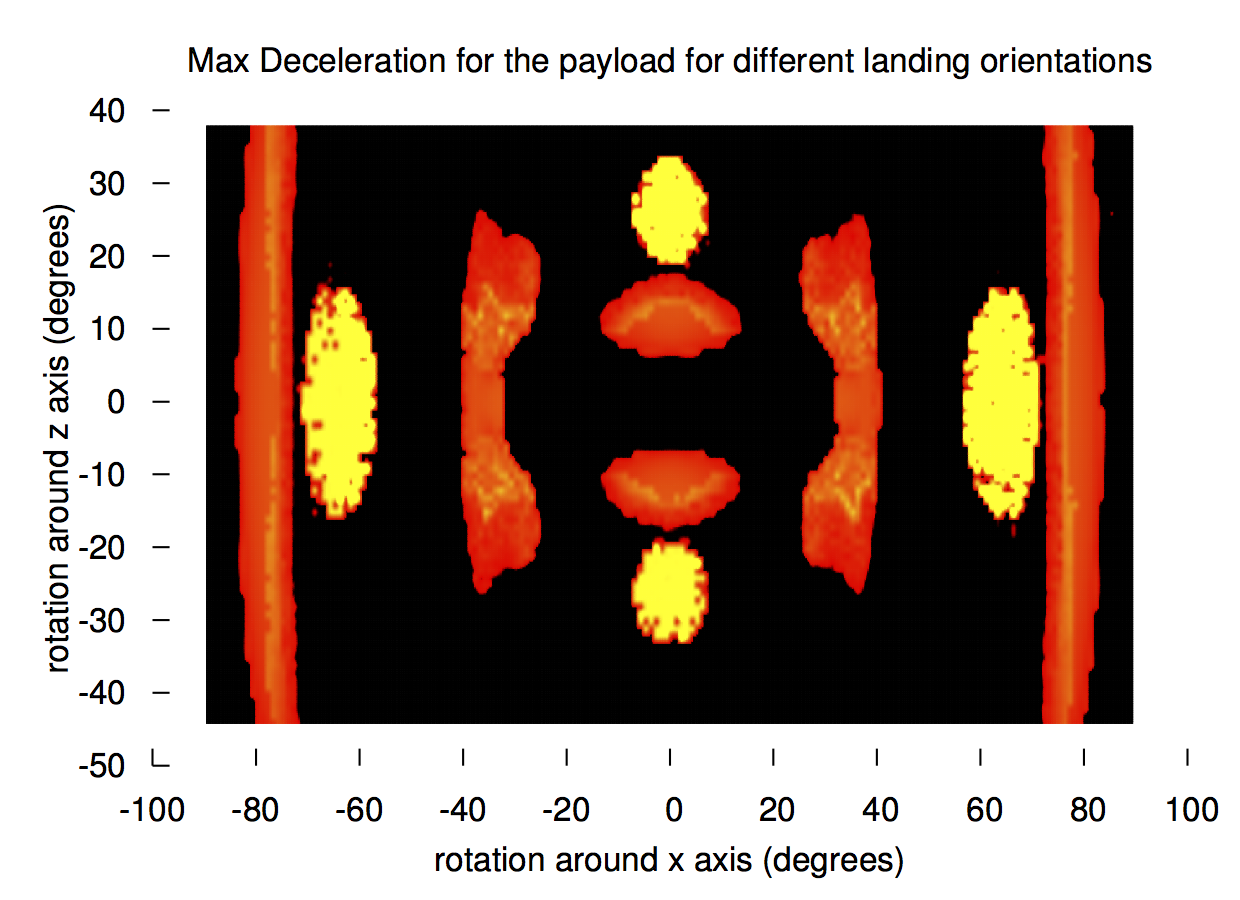
\includegraphics[width=0.8\columnwidth]{tex/images/landing/landingHeatMapRot.png}
   \caption{\em Heat map of the maximum acceleration that the payload encounters for all possible landing orientations. Black areas are safe, colored areas are where the payload does not meet one or both success criteria.}
   \label{fig:landingHeatMapRot}
\end{figure}


\section{Conclusions from Simulation Experiments}
In our landing analysis we developed and cross-validated two different simulation methods that allowed us to explore the capabilities of a tensegrity structure to absorb the forces of landing and to simultaneously protect a delicate payload.  This analysis confirmed that indeed it is possible to do so using a 6-bar tensegrity probe while maintaining maximum decelerations experienced by the instrument-containing payload to forces less than 25G, despite the structure landing at 15 m/s (which is greater than terminal velocity on Titan).   Comparing this to the Huygens probe's landing acceleration of \(32G\) \cite{lorenz1994huygens}, the tensegrtiy probe will have a \(43\% \) reduction in \(G\) forces experienced by the scientific payload, despite the Huygens probe's use of parachutes to land at 1/3 of the speed of our tensegrity probe.
